\chapter{Projekt- und Qualitätsmanagement}
	\label{cap:projectmanagement}
	
	Zur Verwaltung des Projektes hat das Projektteam ein Jira eingesetzt.
	
	\section{Projektmanagement}
		Zur Grobplanung und zur Planung der Milestones wurden Jira-Versions eingesetzt.
		
		\begin{figure}[H]
			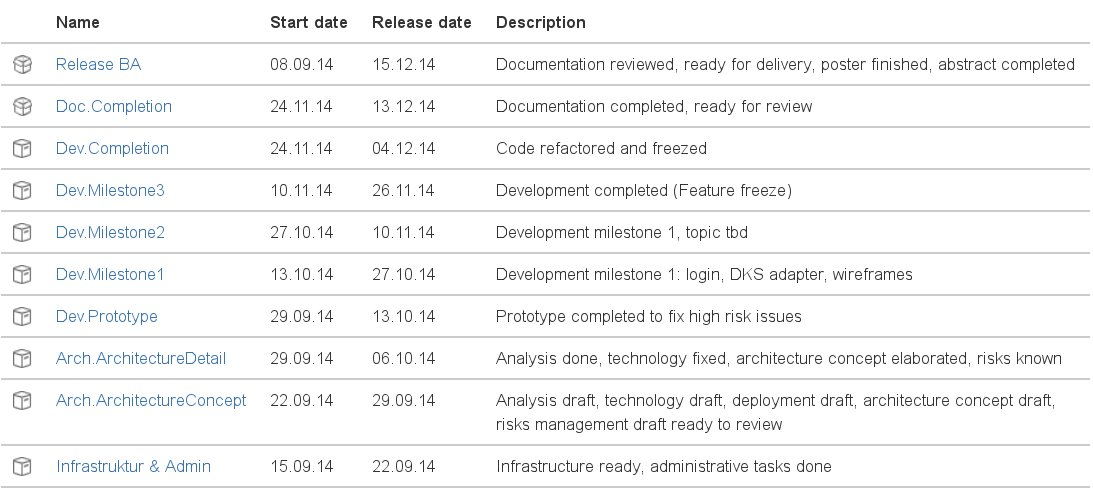
\includegraphics[width=\textwidth]{projectPlan/media/img/jiraVersions.jpg}
			\centering
			\caption{Jira Versions/Milestones}
			\label{fig:jiraVersions}
		\end{figure}
		
		Features haben wir in Zusammenarbeit mit dem Vertreter der Kundengruppe priorisiert und daraus resultierende Issues Milestones zugeordnet.
		Zur Strukturierung haben wir zusätzlich Labels eingesetzt.
		
		\begin{figure}[H]
			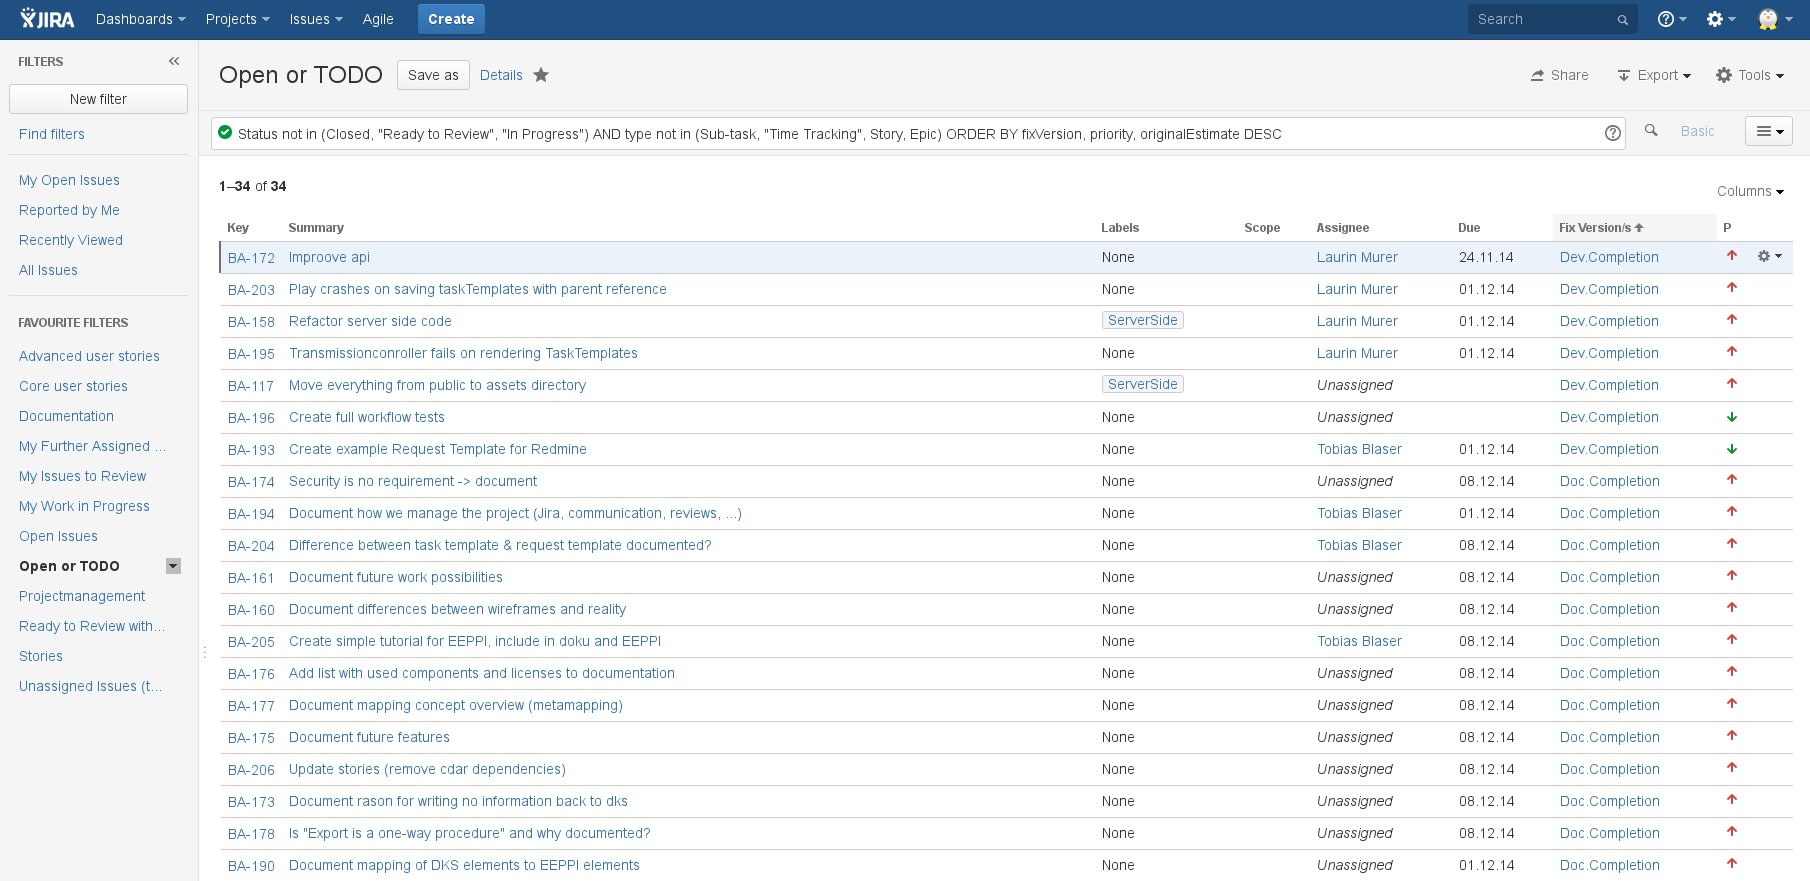
\includegraphics[width=\textwidth]{projectPlan/media/img/jiraIssuesOpenOrTodo.jpg}
			\centering
			\caption{Jira Issues, sortiert nach Version}
			\label{fig:jiraIssuesOpenOrTodo}
		\end{figure}
		
		Anhand den geschätzten Aufwänden
		pro Issue und der zur Verfügung stehenden Zeit eines Milestones haben wir jeweils eine Milestoneplanung durchgeführt.		
		Dabei haben wir maximal 2/3 der zur Verfügung stehenden Zeit für
		Issues eingeplant und den Rest für Unvorhergesehenes, 
		Meetings und Planung vorgesehen.
		
		\begin{figure}[H]
			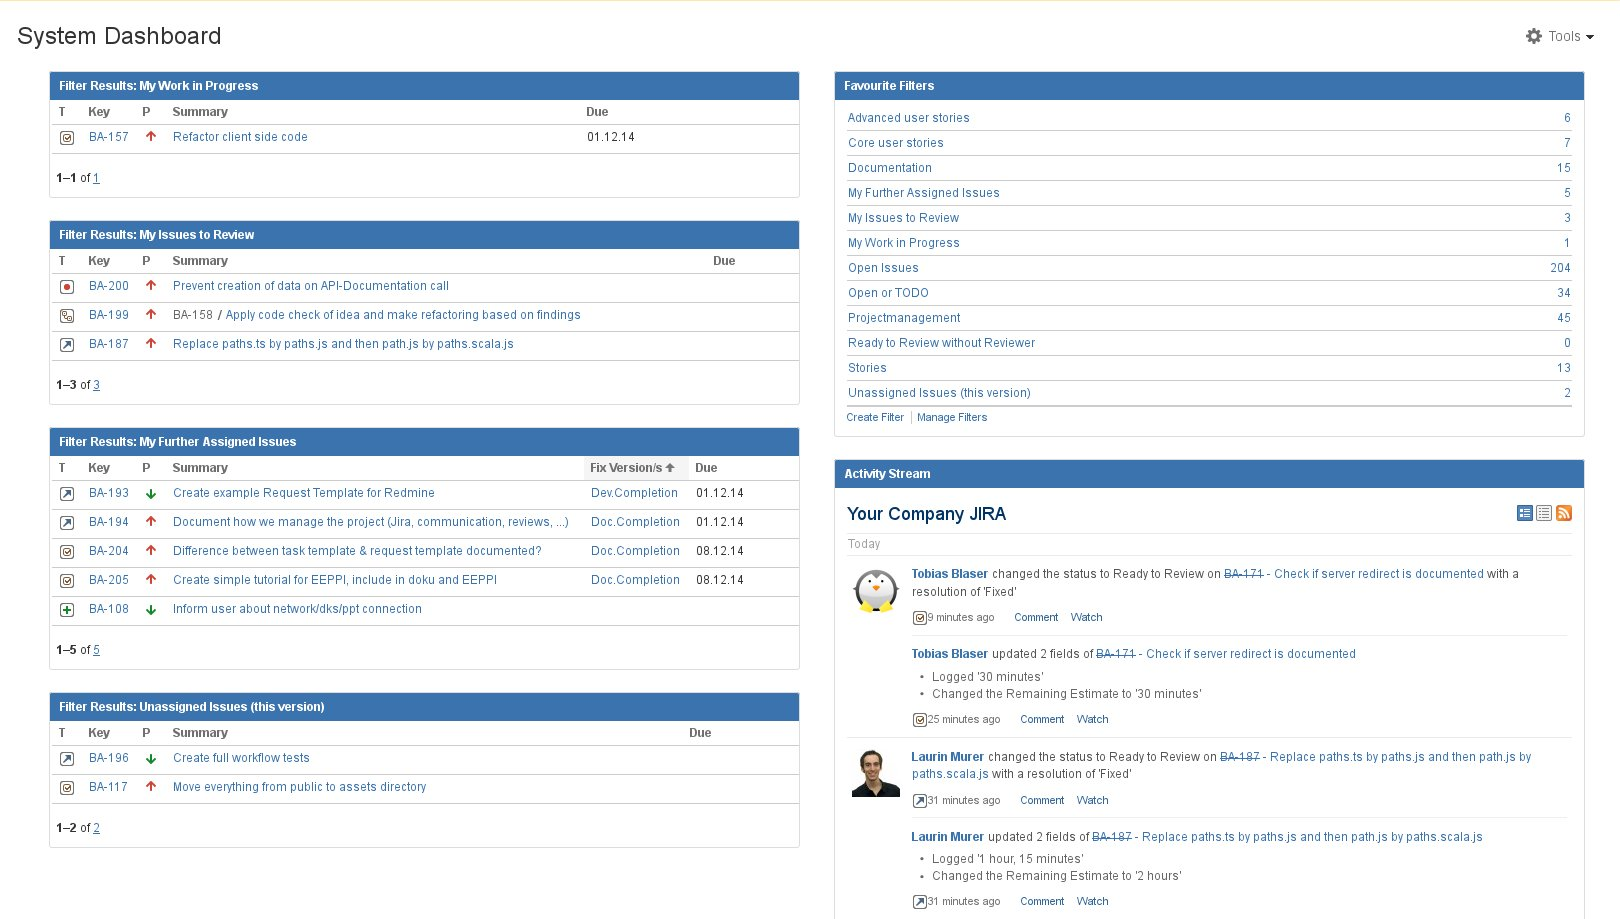
\includegraphics[width=\textwidth]{projectPlan/media/img/jiraDashBoard.jpg}
			\centering
			\caption{Jira Dashboard}
			\label{fig:jiraDashBoard}
		\end{figure}
		
		Jira bietet anpassbare Dashboards, 
		die einen Überblick über das laufende Projekt bieten.
		
		Der Activity Stream von Jira sowie die Git History ermöglichten es uns auf einfache Weise nachzuvollziehen,
		an was der Teampartner in den letzten Stunden gearbeitet hat. 
		Dies senkt den Kommunikationsaufwand und die Notwendigkeit,
		jederzeit gemeinsam an einem Ort zu arbeiten.
		
		\begin{figure}[H]
			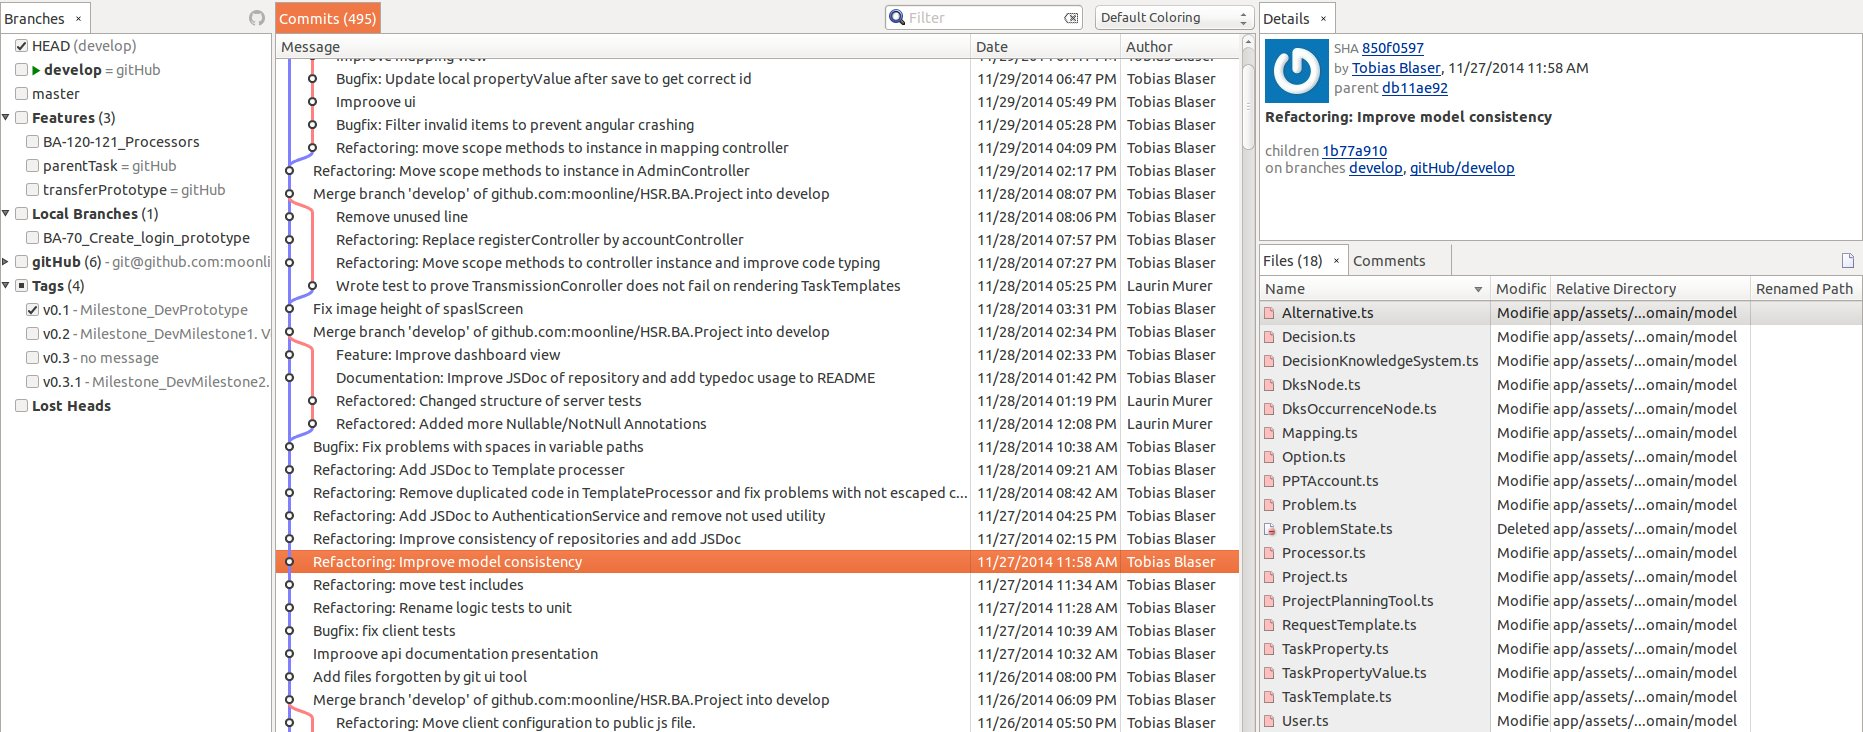
\includegraphics[width=\textwidth]{projectPlan/media/img/gitHistory.jpg}
			\centering
			\caption{Git History in SmartGit}
			\label{fig:gitHistory}
		\end{figure}
		
		Für grössere Features haben wir Git Flow Featurebranches eingesetzt.
		Für Releases entsprechend Releasebranches.
		Zusätzliche haben wir die Funktion "'Releases"' von Github
		zum Hinzufügen von fertigen Builds zu Releases genutzt.
		
		\begin{figure}[H]
			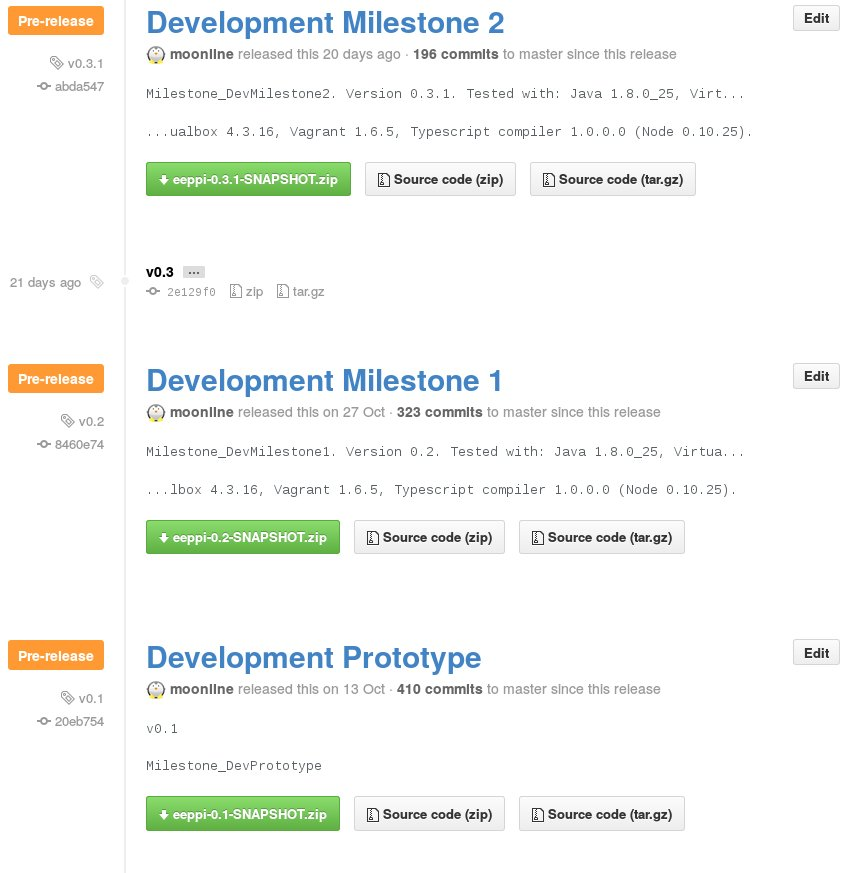
\includegraphics[width=0.5\textwidth]{projectPlan/media/img/githubReleases.jpg}
			\centering
			\caption{Github Releases mit Build-Archives}
			\label{fig:githubReleases}
		\end{figure}
	
		
	\section{Qualitätssicherung}
		Um sicherzustellen, dass keine Issues geschlossen werden,
		ohne dass die Arbeit einem Review unterzogen wurde,
		haben wir den Issue Workflow im Jira entsprechend gestaltet.		
		
		\begin{figure}[H]
			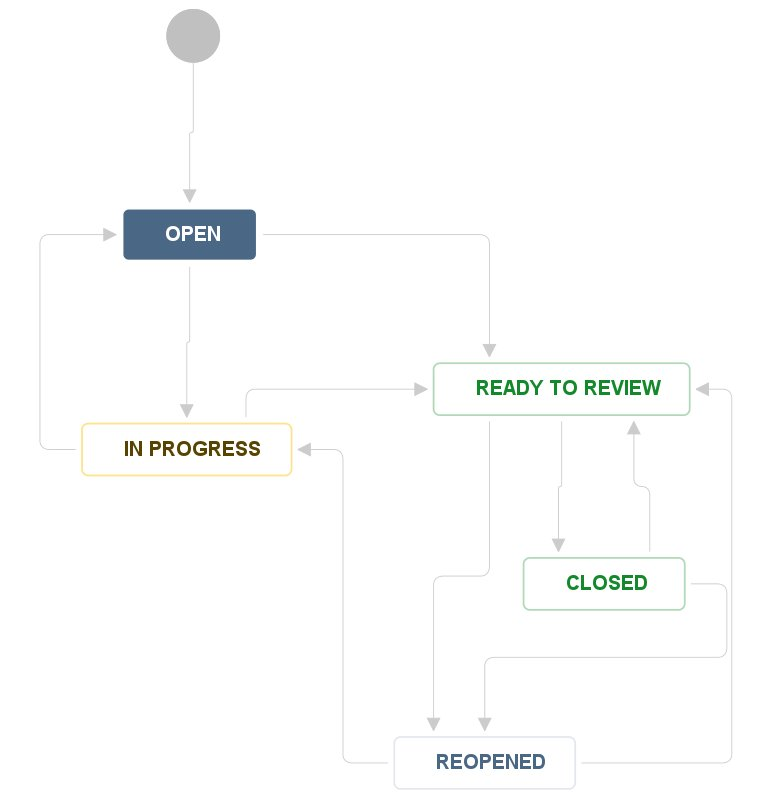
\includegraphics[width=0.5\textwidth]{projectPlan/media/img/jiraIssueWorkflow.jpg}
			\centering
			\caption{Angepassten Jira Issue-Workflow}
			\label{fig:jiraIssueWorkflow}
		\end{figure}
		
		Fertig gestellte Issues müssen immer dem andern Teammitglied
		zum Review gesandt werden und tauchen entsprechend auf dessen
		Dashboard als "'Ready to Review"' auf.
		
		Es geht dabei nicht darum, 
		für jeden erledigten Issue den kompletten Code des Andern anzusehen, 
		sondern das Resultat grob anzuschauen und eventuell
		Edge-Cases\footnote{Spezialfälle, bezogen auf Input Daten oder 
		Workflows der grafischen Oberfläche} zu prüfen. 
		Ein komplettes Code Review jedes Issues wäre zeitlich nicht verhältnismässig.
		
		% TODO:explain used tools in infrastructure
		\section{Testkonzept}
		
			Um zuverlässig alle notwenigen Bereiche mit Tests abzudecken, 
			werden folgende Tests durchgeführt:
			
			\begin{description}
				\item[Unit (Unit- /Logiktests)] Tests, die eine einzelne Klasse, 
					Service oder Komponente testen. 
					Andere Klassen sind nur soweit Teil des Tests, 
					wie dies aufgrund der Abhängigkeiten notwendig ist.
				\item[Integration (Integrationstests)] Tests, die das Zusammenspiel zwischen Klassen, 
					Komponenten und Services testen. 
					Diese Tests können über mehrere Layers bis mehrere Tiers laufen.
					Alle API-Aufrufe werden mit solchen Tests getestet.
				\item[Behaviour (Verhaltenstests)] Gross-Integrationstests, 
					die über alle Tiers und Layers laufen. 
					Diese Tests testen Workflows von der Persistenz 
					bis zur grafischen Ausgabe im Userinterface. 
					Dazu wird mit Selenium ein Browser gestartet und dessen Ausgabe analysiert.
					%TODO: evtl. User-Stories testen
			\end{description}
		
	\section{Metriken}
	Zur Analyse von \eeppi\ haben wir drei verschiedene Arten von Metriken erstellt.
	Die erste zeigt den Umfang des Projekts,
	zweitere wie gut wir getestet haben
	und die dritte gitb Auskunft über die Code Qualität.
	
	Auf dem Client wurde mit TypeScript entwickelt, dieses wurde zu JavaScript kompiliert.
	Die Metriken über den Code Umfang wurden für den Clientteil mit den TypeScript-Dateien durchgeführt,
	die restlichen Metriken aufgrund der mangelnden Verfügbarkeit an Tools für TypeScritpt direkt mit dem JavaScript.
	Dies hat soweit einen Einfluss, das die Qualität des von TypeScript erzeugten Codes die Messung beeinflusst.
	
	\subsection{Umfang}
	Total setzt sich \eeppi\ aus gut 25'000 Zeilen Code zusammen, inklusive Leerzeilen, Kommentaren, Konfigurationsdaten und Code von anderen Entwicklern.
	Die Zusammensetzung ist in Abb. \ref{fig:TotalSLOC} zu sehen.
	\begin{figure}[H]
		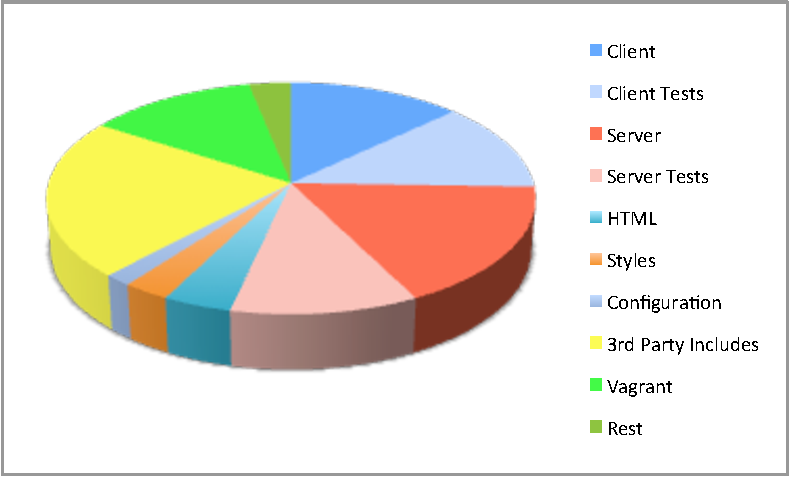
\includegraphics[width=\largeThird\textwidth]{projectPlan/media/img/totalSLOC.pdf}
		\centering
		\caption{Total SLOC (Source Lines of Code)}
		\label{fig:TotalSLOC}
	\end{figure}
	
	Gut die Hälfte des Umfangs entfällt dabei auf unsern Client- und Servercode und seine Tests.
	Ein weiterer grosser Anteil stellen die externen Libraries und Frameworks (22\%),
	sowie die Daten für die Initialkonfiguration der Vagrant-Umgebungen.
	Die restlichen 12\% des Projektes setzen sich zusammen aus Konfiguration, Templates für die Benutzeroberfläche und Styles.
	
	Wird der Hauptteil von \eeppi\ betrachtet (effektiver ausführbarer Code Server- und Client),
	ist zu sehen, dass die Server- und Client in der gleichen Grössendimension liegen.
	Dies war zu erwarten, da sie auch den gleichen Umfang der Daten verarbeiten.
	
	Auch die Tests liegen in der gleichen Grössenordnung.
	Allerdings sind im Client Test Code viele Zeilen an Initialisierungsdaten enthalten zum mocken\footnote{Das verwendete Test-Framework Angular Jasmine erlaubt das simulieren (mocken) der REST Schnittstelle} der Schnittstellenaufrufe. 
	Die effektive Grösse der Client Tests liegt ca. 25-30\% tiefer.
	
	Die detailierte Aufteilung und genaue Anzahl der SLOC (Source Lines of Code) der eigenen Codeteile ist in Abbildung\ \ref{fig:serverClientSLOC} zu sehen.
	\begin{figure}[H]
		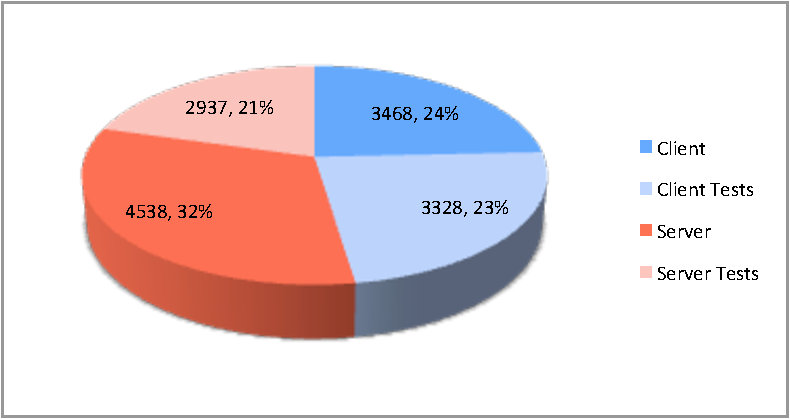
\includegraphics[width=\largeThird\textwidth]{projectPlan/media/img/serverClientSLOC.pdf}
		\centering
		\caption{Vergleich SLOC (Source Lines of Code) auf Server und Client inklusive Tests}
		\label{fig:serverClientSLOC}
	\end{figure}

	\subsection{Test Coverage}
	Sowohl auf dem Server als auch auf dem Client sind wir mehrheitlich nach TDD (Test Driven Development) vorgegangen,
	dementsprechend hoch ist die Testabdeckung.
	Ziel war von Anfang an nicht 100\% Testabdeckung zu erreichen, sondern die wichtigsten Funktionen zu testen.
	
	\begin{figure}[H]
		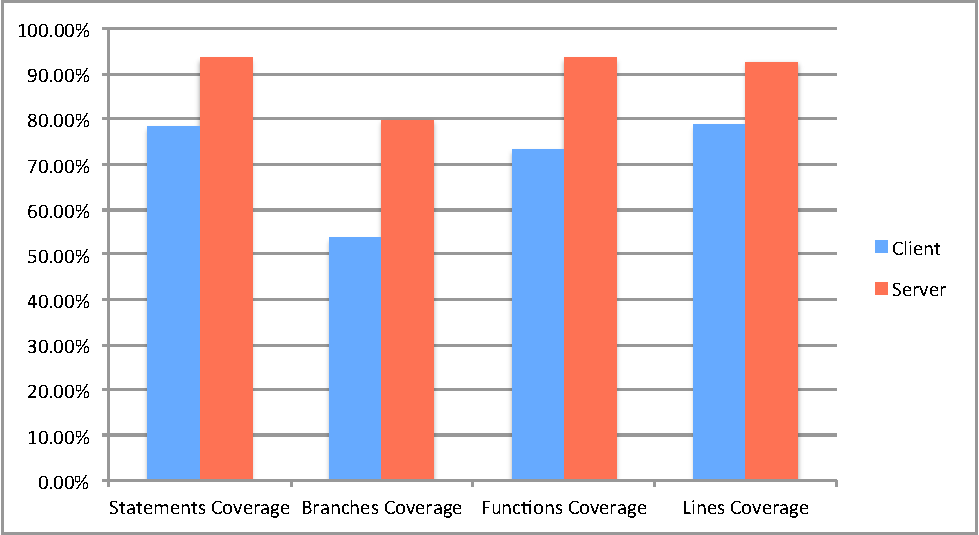
\includegraphics[width=\textwidth]{projectPlan/media/img/coverage.pdf}
		\centering
		\caption{Testabdeckung auf dem Server und dem Client}
		\label{fig:coverage}
	\end{figure}
	Abb. \ref{fig:coverage} zeigt die Testabdeckung auf.
	Es ist zu sehen, dass auf dem Server die Testabdeckung höher ist als auf dem Client,
	aber auch auf dem Client sind die zentralen und wichtigen Elemente gut abgedeckt.
	
	\subsection{Qualität}
	Die Codequalität ohne grosse Verfälschung zu messen ist eine grosse Herausforderung.
	Hier zeigt sich der erwähnte Einfluss des generierten JavaScipts besonders stark. TypeScipt generiert viele anonyme, direkt ausgeführte Funktionen, die der Kapselung des Codes dienen. 
	Der so erzeugte Code drückt die Metriken in die Höhe. Trotzdem lassen sich einige Aussagen treffen anhand der gemessenen Daten.
	
	Wir haben die wichtigsten Kennzahlen evaluiert,
	so die Anzahl der Logical LOC (Anzahl Zeilen pro Methode), die Anzahl der Parameter und die Cyclomatic Complexity\footnote{Komplexitätswert der die Operationen pro Methode repräsentiert \url{http://www.aivosto.com/project/help/pm-complexity.html}}.
	
	\begin{figure}[H]
		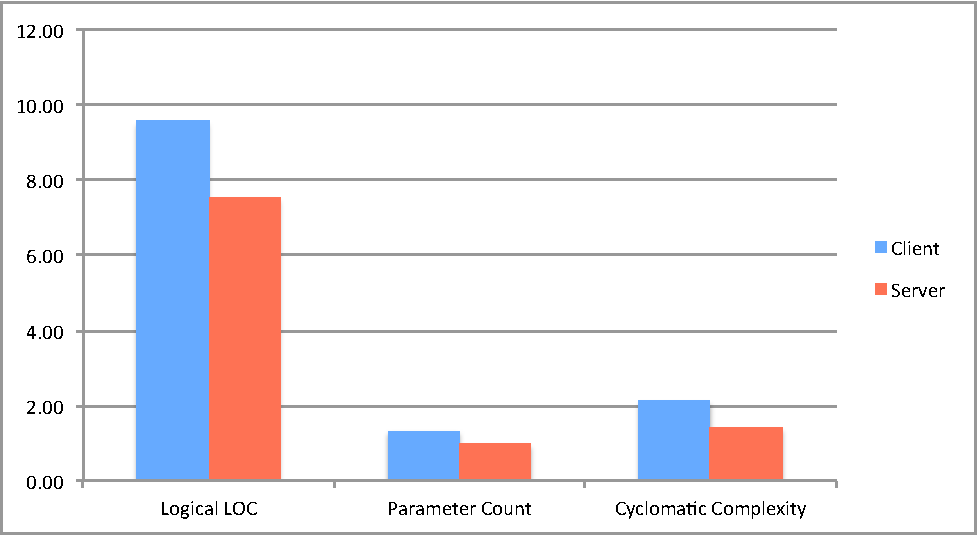
\includegraphics[width=\textwidth]{projectPlan/media/img/methodComplexityOverview.pdf}
		\centering
		\caption{Überblick Komplexitätskennwerte pro Methode (Durchschnitt)}
		\label{fig:methodComplexityOverview}
	\end{figure}
	
	In Abb. \ref{fig:methodComplexityLLOC} ist die Anzahl der logischen Zeilen Code pro Methode ausgewiesen.
	Gut sichtbar, dass auf dem Server 35\% aller Methoden drei logische Codezeilen aufweisen.
	Spannend ist die grosse Spitze beim Client gegen das Ende der Grafik.
	Sie steht für die langen, von TypeScript erzeugten Methoden, die beispielsweise ganze Prototypen wrappen und der Kapselung dienen.
	
	Zusammengefasst kann man sagen, das die Mehrheit der Methoden mit drei bis sieben Zeilen Code auskommen und einige Wenige mehr als 20 Zeilen aufweisen.
	
	\begin{figure}[H]
		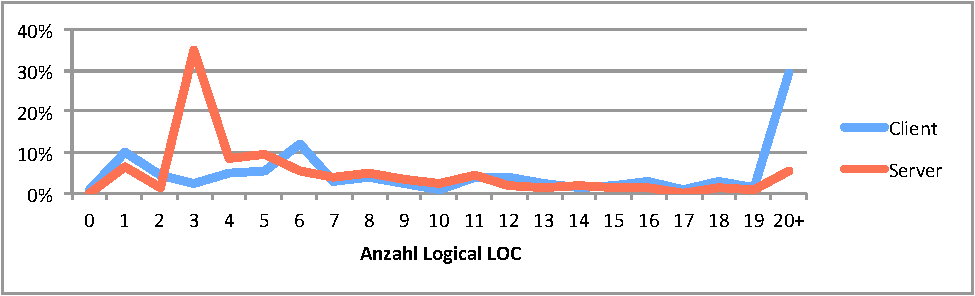
\includegraphics[width=\textwidth]{projectPlan/media/img/methodComplexityLLOC.pdf}
		\centering
		\caption{Anzahl Logical LOC pro Methode}
		\label{fig:methodComplexityLLOC}
	\end{figure}
	
	In Abb. \ref{fig:methodComplexityParameterCount} wird die Häufigkeit der Anzahl Methoden Parameter aufgezeigt.
	Gut erkennbar die Tatsache, dass sowohl auf dem Server, wie auch auf dem Client,
	die meisten Methoden keinen oder nur einen einzigen Parameter besitzen.
	
	
	\begin{figure}[H]
		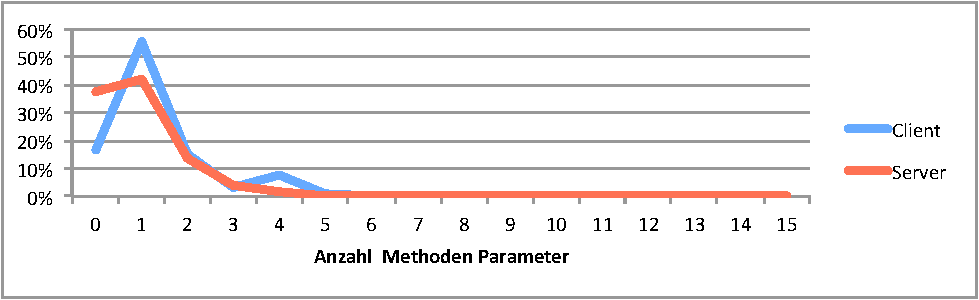
\includegraphics[width=\textwidth]{projectPlan/media/img/methodComplexityParameterCount.pdf}
		\centering
		\caption{Anzahl Parameter pro Methode}
		\label{fig:methodComplexityParameterCount}
	\end{figure}
	Abschliessend ist die Cyclomatic Complexity in Abb. \ref{fig:methodComplexityCyclomaticComplexity} aufgezeichnet.  
	Sie beschreibt, wie viele Operationen eine Methode enthält.
	Beim Server repräsentiert die Spitze bei eins die Getter und Setter,
	diese sind beim Client so nicht zu sehen.
	JavaScript erlaubt das anlegen von Methoden für direkten Property-Zugriff, womit für alle nicht-Private Property Setter und Getter entfallen.
	Die Tatsache, das die Mehrheit der Objekte auf dem Client innerhalb der Templates verwendet wird, erfordert viele Public-Properties.
	Zusätzlich bedingt sind viele Public-Properties aufgrund der Factory,
	die Prototypen anhand der Übertragenen Daten zusammenbaut.	
	
	
	\begin{figure}[H]
		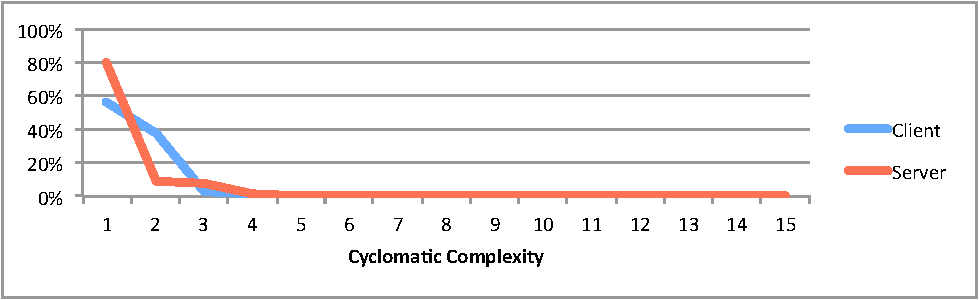
\includegraphics[width=\textwidth]{projectPlan/media/img/methodComplexityCyclomaticComplexity.pdf}
		\centering
		\caption{Cyclomatic Complexity pro Methode}
		\label{fig:methodComplexityCyclomaticComplexity}
	\end{figure}
	
	
	\subsection{Fazit}
		\eeppi\ weist einen ansehnlichen Umfang auf und auch eine gute Testabdeckung.
		Die effektive Höhe  der Codequalität lässt sich jedoch nur schwer eruieren.	
		
		Ungefähr in der Mitte des Projekts hat ein Mitarbeiter des IFS\footnote{Institut für Software, HSR Hochschule für Technik Rapperswil, \url{http://www.ifs.hsr.ch}} einen Codereview durchgeführt und positive Bilanz gezogen.
		Zusätzlich sind aufgrund dieses Feedbacks Verbesserungen in den Code eingeflossen.
		
		Maurice Halstead hat eine Softwaremetrik entworfen,
		welche die Komplexität der Software berechnet und davon ausgehend einige Kennzahlen liefert.
		Eine davon ist die "'Halstead Bugs"', sie gibt die Fehlerkomplexität an,
		also wie viele Fehler die Software aufgrund der berechneten Komplexität und Grösse statistisch ungefähr enthalten könnte.
		Das heisst aber nicht, dass die Software so viele Fehler enthält,
		sondern die Abstraktion mit Bugs ist nur für das bessere Verständnis der Grössenordnung gedacht.
		
		\begin{figure}[H]
			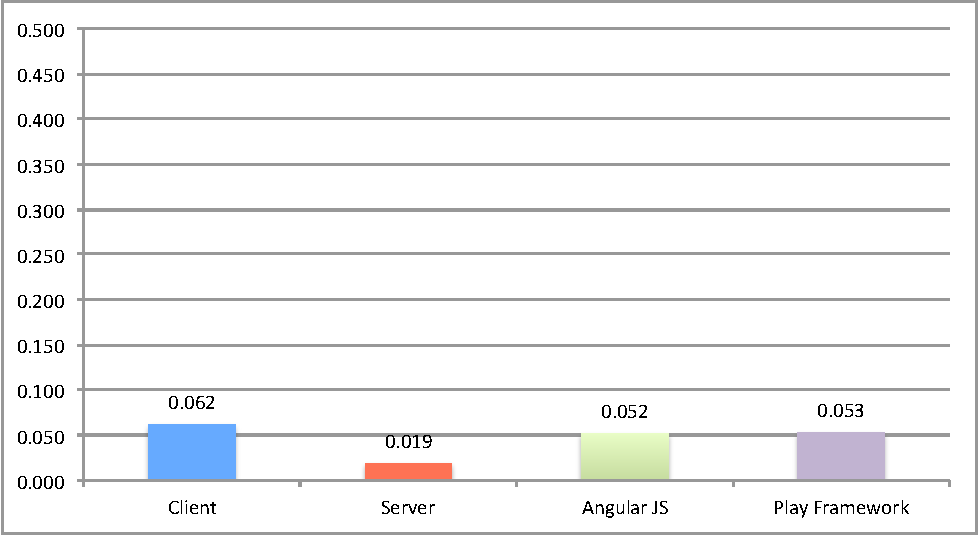
\includegraphics[width=\textwidth]{projectPlan/media/img/halsteadBugsPerMethod.pdf}
			\centering
			\caption{Halstead Bugs pro Methode}
			\label{fig:halsteadBugsPerMethod}
		\end{figure}
		
		In Abbildung\ \ref{fig:halsteadBugsPerMethod} ist diese Komplexitätsgrösse verglichen mit zwei der durch \eeppi\ eingesetzten Frameworks.
		Der Client weist in etwa die gleiche Komplexität auf,
		wie die beiden Frameworks, der Server eine geringere.
		
		Zieht man in Betracht, das ein Grossteil der Komplexität auf dem Client der Erzeugung des TypeScriptes geschuldet ist, so wird sich die effektive Komplexität auf dem Client im Bereich zwischen dem Server und Angular bewegen, also zwischen 0.02 und 0.05. 
		
	\subsubsection{Typescript}
	Die Art des von Typescript erzeugten Codes wirft die Frage auf, was TypeScript bringt und ob es sich gelohnt hat.
	
	Aus unserer Sicht hat sich der Einsatz von TypeScript sehr gelohnt. 
	Viele Fehler haben wir dadurch bereits zur Kompilierzeit gefunden und nicht erst zur Laufzeit.
	Der Source Code ist strukturierter, modularisierter, gekapselter und trotzdem lesbarer als vergleichbarer JavaScript Code dies wäre.
	Für Wartung und Weiterentwicklung spielt insofern der erzeugte JavaScript Code nur eine untergeordnete Rolle. Daher überwiegen die Vorteile von TypeScript ganz klar.
	
